%\documentclass{article}
\documentclass[]{article}
\usepackage{bm}
\usepackage{amsmath}
\usepackage{amsfonts}
\usepackage{natbib}
\usepackage{graphicx}
\bibliographystyle{unsrtnat}

\begin{document}

\section{Stimulus Experiments}


\begin{itemize}
	\item What is the research question?
	\item Stimulus checks. Is there a delay - much less so this time around.
	\item Payroll tax cut
	\subitem Is this passed through to workers? Obama stimulus was 2\% ONLY on the employee side
	\subitem Not applicable to the unemployed. 
	\subitem Not applicable to retirees (we don't have lifecycle at the moment).
	\subitem Not applicable to incomes over \$130,000 or there about
	\subitem Is the motivation for a payroll tax cut really consumption stimulus, or is it to encourage more employment (both from worker and employer)
	\item Unemployment benefit extension
	\subitem 26 weeks is standard, Obama increased by 20 weeks
	\item Automatic stabilizer
	\subitem Something like the Sahm rule with stimulus checks going out automatically if ``the three-month moving average of the national unemployment rate (U3) rises by 0.50 percentage points or more relative to its low during the previous 12 months.''
\end{itemize}

General comments
\begin{itemize}
	\item Current focus is on duration of stimulus, rather than targeting specific household characteristics. Is that what we want? There is a argument that stimulus should be ``large and fast'' to get out of a recession, which could come out of a NK type framework. Do we want to make this a focus?
	\item Is a NK framework the correct one here? New Fed consensus statement focuses on employment shortfall, suggesting more of a one-sided model framework.
	\item How do we judge the appropriateness of a policy? Are we going to do welfare analysis?
	\item How do we handle general equilibrium, particularly at the effective lower bound?
\end{itemize}

	\begin{figure} 
	\begin{centering}
		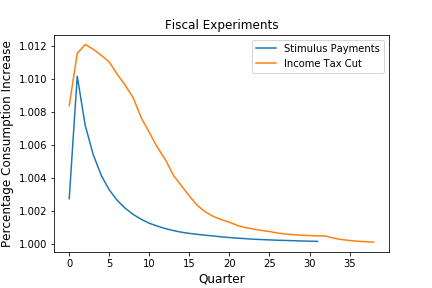
\includegraphics[scale=0.85]{./Figures/FiscalExperiments.png}
		\caption{Fiscal Stimulus Experiments}
		\label{fig:Fiscal_experiments}
	\end{centering}
	\end{figure}

\end{document}
